\documentclass[ignorenonframetext,]{beamer}
\setbeamertemplate{caption}[numbered]
\setbeamertemplate{caption label separator}{: }
\setbeamercolor{caption name}{fg=normal text.fg}
\beamertemplatenavigationsymbolsempty
\usepackage{lmodern}
\usepackage{amssymb,amsmath}
\usepackage{ifxetex,ifluatex}
\usepackage{fixltx2e} % provides \textsubscript
\ifnum 0\ifxetex 1\fi\ifluatex 1\fi=0 % if pdftex
  \usepackage[T1]{fontenc}
  \usepackage[utf8]{inputenc}
\else % if luatex or xelatex
  \ifxetex
    \usepackage{mathspec}
  \else
    \usepackage{fontspec}
  \fi
  \defaultfontfeatures{Ligatures=TeX,Scale=MatchLowercase}
\fi
% use upquote if available, for straight quotes in verbatim environments
\IfFileExists{upquote.sty}{\usepackage{upquote}}{}
% use microtype if available
\IfFileExists{microtype.sty}{%
\usepackage{microtype}
\UseMicrotypeSet[protrusion]{basicmath} % disable protrusion for tt fonts
}{}
\newif\ifbibliography
\hypersetup{
            pdftitle={Stepwise Regression with Negatively Correlated Covariates},
            pdfauthor={Riley Ashton},
            pdfborder={0 0 0},
            breaklinks=true}
\urlstyle{same}  % don't use monospace font for urls
\usepackage{color}
\usepackage{fancyvrb}
\newcommand{\VerbBar}{|}
\newcommand{\VERB}{\Verb[commandchars=\\\{\}]}
\DefineVerbatimEnvironment{Highlighting}{Verbatim}{commandchars=\\\{\}}
% Add ',fontsize=\small' for more characters per line
\usepackage{framed}
\definecolor{shadecolor}{RGB}{248,248,248}
\newenvironment{Shaded}{\begin{snugshade}}{\end{snugshade}}
\newcommand{\KeywordTok}[1]{\textcolor[rgb]{0.13,0.29,0.53}{\textbf{#1}}}
\newcommand{\DataTypeTok}[1]{\textcolor[rgb]{0.13,0.29,0.53}{#1}}
\newcommand{\DecValTok}[1]{\textcolor[rgb]{0.00,0.00,0.81}{#1}}
\newcommand{\BaseNTok}[1]{\textcolor[rgb]{0.00,0.00,0.81}{#1}}
\newcommand{\FloatTok}[1]{\textcolor[rgb]{0.00,0.00,0.81}{#1}}
\newcommand{\ConstantTok}[1]{\textcolor[rgb]{0.00,0.00,0.00}{#1}}
\newcommand{\CharTok}[1]{\textcolor[rgb]{0.31,0.60,0.02}{#1}}
\newcommand{\SpecialCharTok}[1]{\textcolor[rgb]{0.00,0.00,0.00}{#1}}
\newcommand{\StringTok}[1]{\textcolor[rgb]{0.31,0.60,0.02}{#1}}
\newcommand{\VerbatimStringTok}[1]{\textcolor[rgb]{0.31,0.60,0.02}{#1}}
\newcommand{\SpecialStringTok}[1]{\textcolor[rgb]{0.31,0.60,0.02}{#1}}
\newcommand{\ImportTok}[1]{#1}
\newcommand{\CommentTok}[1]{\textcolor[rgb]{0.56,0.35,0.01}{\textit{#1}}}
\newcommand{\DocumentationTok}[1]{\textcolor[rgb]{0.56,0.35,0.01}{\textbf{\textit{#1}}}}
\newcommand{\AnnotationTok}[1]{\textcolor[rgb]{0.56,0.35,0.01}{\textbf{\textit{#1}}}}
\newcommand{\CommentVarTok}[1]{\textcolor[rgb]{0.56,0.35,0.01}{\textbf{\textit{#1}}}}
\newcommand{\OtherTok}[1]{\textcolor[rgb]{0.56,0.35,0.01}{#1}}
\newcommand{\FunctionTok}[1]{\textcolor[rgb]{0.00,0.00,0.00}{#1}}
\newcommand{\VariableTok}[1]{\textcolor[rgb]{0.00,0.00,0.00}{#1}}
\newcommand{\ControlFlowTok}[1]{\textcolor[rgb]{0.13,0.29,0.53}{\textbf{#1}}}
\newcommand{\OperatorTok}[1]{\textcolor[rgb]{0.81,0.36,0.00}{\textbf{#1}}}
\newcommand{\BuiltInTok}[1]{#1}
\newcommand{\ExtensionTok}[1]{#1}
\newcommand{\PreprocessorTok}[1]{\textcolor[rgb]{0.56,0.35,0.01}{\textit{#1}}}
\newcommand{\AttributeTok}[1]{\textcolor[rgb]{0.77,0.63,0.00}{#1}}
\newcommand{\RegionMarkerTok}[1]{#1}
\newcommand{\InformationTok}[1]{\textcolor[rgb]{0.56,0.35,0.01}{\textbf{\textit{#1}}}}
\newcommand{\WarningTok}[1]{\textcolor[rgb]{0.56,0.35,0.01}{\textbf{\textit{#1}}}}
\newcommand{\AlertTok}[1]{\textcolor[rgb]{0.94,0.16,0.16}{#1}}
\newcommand{\ErrorTok}[1]{\textcolor[rgb]{0.64,0.00,0.00}{\textbf{#1}}}
\newcommand{\NormalTok}[1]{#1}
\usepackage{longtable,booktabs}
\usepackage{caption}
% These lines are needed to make table captions work with longtable:
\makeatletter
\def\fnum@table{\tablename~\thetable}
\makeatother
\usepackage{graphicx,grffile}
\makeatletter
\def\maxwidth{\ifdim\Gin@nat@width>\linewidth\linewidth\else\Gin@nat@width\fi}
\def\maxheight{\ifdim\Gin@nat@height>\textheight0.8\textheight\else\Gin@nat@height\fi}
\makeatother
% Scale images if necessary, so that they will not overflow the page
% margins by default, and it is still possible to overwrite the defaults
% using explicit options in \includegraphics[width, height, ...]{}
\setkeys{Gin}{width=\maxwidth,height=\maxheight,keepaspectratio}

% Prevent slide breaks in the middle of a paragraph:
\widowpenalties 1 10000
\raggedbottom

\AtBeginPart{
  \let\insertpartnumber\relax
  \let\partname\relax
  \frame{\partpage}
}
\AtBeginSection{
  \ifbibliography
  \else
    \let\insertsectionnumber\relax
    \let\sectionname\relax
    \frame{\sectionpage}
  \fi
}
\AtBeginSubsection{
  \let\insertsubsectionnumber\relax
  \let\subsectionname\relax
  \frame{\subsectionpage}
}

\setlength{\parindent}{0pt}
\setlength{\parskip}{6pt plus 2pt minus 1pt}
\setlength{\emergencystretch}{3em}  % prevent overfull lines
\providecommand{\tightlist}{%
  \setlength{\itemsep}{0pt}\setlength{\parskip}{0pt}}
\setcounter{secnumdepth}{0}

\title{Stepwise Regression with Negatively Correlated Covariates}
\author{Riley Ashton}
\date{NSERC Summer 2018}

\begin{document}
\frame{\titlepage}

\begin{frame}{Inspiration}

\begin{itemize}
\tightlist
\item
  \href{https://www.researchgate.net/profile/David_Hamilton23/publication/272559796_Sometimes_R_2_r_2_yx_1_r_2_yx_2_Correlated_Variables_Are_Not_Always_Redundant/links/557825c108ae753637548c1b.pdf}{David
  Hamilton's 1987 Paper} Sometimes \(R^2 > r^2_{yx_1} + r^2_{yx_2}\)
  Correlated Variables Are Not Always Redundant
\item
  Hamilton gave an example when two variables were negatively correlated
  and neither did a good job in explaining the response on their own,
  but together they explained nearly all the variance
  (\(R^2 \approx 1\))
\item
  Could negatively correlated variables impact stepwise regression?
\end{itemize}

\end{frame}

\begin{frame}{Stepwise Selection}

\begin{itemize}
\tightlist
\item
  Greedy algorithm
\item
  Problems if neither variable is significant on its own, but together
  they are both significant
\end{itemize}

\begin{figure}
\centering
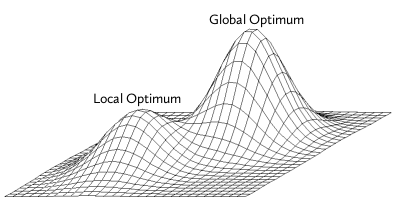
\includegraphics{./local_optimum.png}
\caption{}
\end{figure}

\end{frame}

\begin{frame}{My Paper}

\begin{itemize}
\tightlist
\item
  Algorithms that consider adding highly negatively correlated variables
  together, and additionally any variables correlated with those are
  discussed and tested.
\end{itemize}

\end{frame}

\begin{frame}{Algorithms Overview}

\begin{itemize}
\tightlist
\item
  Step: Name given to the traditional stepwise regression algorithm
\item
  Step2: New algorithm that improves Step by considering treating highly
  negatively correlated covariates as singles or as a block
\item
  Step3: Uses recursion on the blocks of Step2 and the correlation
  between covariates to additionally make larger sized blocks
\end{itemize}

\end{frame}

\begin{frame}[fragile]{Step2 Overview}

\begin{itemize}
\tightlist
\item
  In the case of highly negatively correlated covariate pairs, Step2
  will consider the traditional choices of adding a single variable, but
  also the option of adding both negatively correlated covariates to the
  model (refered to as a block)
\item
  What constitutes a highly negatively block is determined by the
  parameter \texttt{cor\_cutoff}
\item
  In this paper \texttt{cor\_cutoff} = -0.5 was used
\item
  While both Step and Step2 are greedy algorithms, Step2 looks two steps
  ahead at highly negatively correlated covariate pairs
\item
  AIC or BIC is used as the metric for deciding which of the possible
  models is the best at each step
\end{itemize}

\end{frame}

\begin{frame}[fragile]{}

\begin{Shaded}
\begin{Highlighting}[]
\NormalTok{let pairs =}\StringTok{ }\NormalTok{\{(x,y) }\OperatorTok{|}\StringTok{ }\KeywordTok{cor}\NormalTok{(x,y) }\OperatorTok{>}\StringTok{ }\NormalTok{cor_cutoff\}}
\NormalTok{let BIC =}\StringTok{ }\NormalTok{BIC of intercept only model}
\NormalTok{let formula =}\StringTok{ }\NormalTok{intercept only model}

\NormalTok{loop}
\NormalTok{  next_formulas }\OperatorTok{+}\ErrorTok{=}\StringTok{ }\NormalTok{\{(formula }\OperatorTok{+}\StringTok{ }\NormalTok{y) }\OperatorTok{|}\StringTok{ }\NormalTok{y not }\ControlFlowTok{in}\NormalTok{ formula\}}
\NormalTok{  next_formulas }\OperatorTok{+}\ErrorTok{=}\StringTok{ }\NormalTok{\{(formula }\OperatorTok{+}\StringTok{ }\NormalTok{x }\OperatorTok{+}\StringTok{ }\NormalTok{y)}
    \OperatorTok{|}\StringTok{ }\NormalTok{x, y }\ControlFlowTok{in}\NormalTok{ pairs and neither }\ControlFlowTok{in}\NormalTok{ formula\}}

\NormalTok{    let X =}\StringTok{ }\NormalTok{glm fitted }\ControlFlowTok{for}\NormalTok{ each formula }\ControlFlowTok{in}\NormalTok{ next_formulas}
\NormalTok{    let min_BIC =}\StringTok{ }\NormalTok{min BIC }\ControlFlowTok{for}\NormalTok{ the models }\ControlFlowTok{in}\NormalTok{ X}
\NormalTok{    let min_formula =}\StringTok{ }\NormalTok{formula }\ControlFlowTok{for}\NormalTok{ min_info_crit model}

    \ControlFlowTok{if}\NormalTok{(min_info_crit }\OperatorTok{<=}\StringTok{ }\NormalTok{cur_info_crit) \{}
\NormalTok{        cur_info_crit =}\StringTok{ }\NormalTok{min_info_crit}
\NormalTok{        current_formula =}\StringTok{ }\NormalTok{min_formula}
\NormalTok{        next_formulas =}\StringTok{ }\NormalTok{empty list}
\NormalTok{  \} }\ControlFlowTok{else}\NormalTok{ \{return glm fitted with cur_form\}}
\NormalTok{end loop}
\end{Highlighting}
\end{Shaded}

\end{frame}

\begin{frame}[fragile]{Step2 Time Complexity}

\begin{itemize}
\tightlist
\item
  Depends on the choice of \texttt{cor\_cutoff}
\item
  Often within a constant of Step
\item
  Worst case is \texttt{p} times the runtime of Step, where \texttt{p}
  is the number of covariates
\end{itemize}

\end{frame}

\begin{frame}{Step3 Block Selection}

\begin{itemize}
\tightlist
\item
  \(\text{CC}\) := correlation cutoff, \(-1 < \text{CC} < 0\)
\item
  Let \(\text{RCP}\) := positive recursive correlation cutoff,
  \(0 < \text{RCP} < 1\)
\item
  \(\text{RCN}\) := negative recursive correlation cutoff,
  \(-1 < \text{RCN} < 0\)
\item
  In this paper \(\text{CC}\) = -0.5, \(\text{RCP}\) = 0.5,
  \(\text{RCN}\) = -0.5 (arbitrarily)
\item
  Let \(r(x_1,x_2)\) denote the sample correlation between \(x_1\) and
  \(x_2\)
\item
  Let \(S_1\) denote the set of covariates
\item
  Then \(S_2\) denoting the set of highly negatively correlated pairs
  \((x_1,x_2)\) is defined as
  \(S_2 = \{(x_1, x_2) \, | \, x_1 \in S_1 \text{ AND } x_2 \in S_1 \text{ AND } x_1 \neq x_2 \text{ AND } r(x_1,x_2) < \text{CC} \}\)
\item
  Then \(S_3\) denoting the set of triples \((x_1,x_2,x_3)\) is defined
  as
  \(S_3 = \{ (x_1, x_2, x_3) \, | \, (x_1,x_2) \in S_2 \, \land x_3 \, \in S_1 \, \land \, x_3 \notin (x_1, x_2) \land \left(\text{block } x_1 \, x_2 \, x_3 \right) \}\)
\item
  where
  \(\text{block } x \, y \, z = (r(x,z) < \text{RCN}) \lor (r(x,z) > \text{RCP}) \lor (r(y,z) < \text{RCN}) \lor (r(y,z) > \text{RCP})\)
\end{itemize}

\end{frame}

\begin{frame}{Step3 Time Complexity}

\begin{itemize}
\tightlist
\item
  Depends on the choice of algorithm parameters
\item
  Hyperparameters can be chosen to make runtime within a constant of
  Step
\item
  Worst case with a maximum block size of \(\text{mbs}\) is
  \(\mathcal O\left( p ^ {(\text{mbs}-1)}\right)\) times greater than
  Step
\end{itemize}

\end{frame}

\begin{frame}{Linear Model Setup}

\begin{itemize}
\tightlist
\item
  \(\mathbf Y = \beta_0 + \beta_1 \mathbf X_1 + \beta_2 \mathbf X_2 + \cdots + \epsilon\)
\item
  \(\mathbf X_i\) are correlated, centred random normal variables
\item
  Intercept (\(\beta_0 = 9\))
\item
  \(\epsilon \sim \mathcal N(\mu = 0, \sigma = 1)\)
\item
  \(n = 100\)
\item
  1000 Simulations
\end{itemize}

\end{frame}

\begin{frame}{Model 1 : Two negatively correlated}

This model is designed to show the advantage of Step2 over Step

\[ \boldsymbol{\Sigma} =\begin{bmatrix}
1   &-0.8 & 0 & 0 & 0 & 0 \\
-0.8& 1   & 0 & 0 & 0 & 0 \\
0   & 0   & 1 & 0 & 0 & 0 \\
0   & 0   & 0 & 1 & 0 & 0 \\
0   & 0   & 0 & 0 & 1 & 0 \\
0   & 0   & 0 & 0 & 0 & 1
\end{bmatrix} \hspace{10pt}
\hspace{20pt}
\boldsymbol{\beta} = \begin{bmatrix} 1 \\ 1 \\ 0 \\ 0 \\ 0 \\ 0 \end{bmatrix}\]

\end{frame}

\begin{frame}{Model 2: Three Negatively Correlated}

This model is designed to show the advantage of Step3 over Step2 and
Step

\[\boldsymbol{\Sigma} = \begin{bmatrix}
1     & -0.8  & 0.25  & 0 & 0 & 0 & 0 & 0 & 0 & 0 \\
-0.8  & 1     & -0.75 & 0 & 0& 0 & 0 & 0 & 0 & 0 \\
0.25  & -0.75 & 1     & 0 & 0& 0 & 0 & 0 & 0 & 0 \\
0     & 0     & 0     & 1 & 0& 0 & 0 & 0 & 0 & 0 \\
0     & 0     & 0     & 0 & 1 & 0 & 0 & 0 & 0 & 0 \\
0     & 0     & 0     & 0 & 0 & 1 & 0 & 0 & 0 & 0 \\
0     & 0     & 0     & 0 & 0 & 0 & 1 & 0 & 0 & 0 \\
0     & 0     & 0     & 0 & 0 & 0 & 0 & 1 & 0 & 0 \\
0     & 0     & 0     & 0 & 0 & 0 & 0 & 0 & 1 & 0 \\
0     & 0     & 0     & 0 & 0 & 0 & 0 & 0 & 0 & 1 \\
\end{bmatrix}
\hspace{10pt}
\hspace{20pt}
\boldsymbol{\beta}  =
\begin{bmatrix} 1 \\ 1 \\ 1 \\ 0 \\ 0 \\ 0 \\ 0 \\ 0 \\ 0 \\ 0
\end{bmatrix}\]

\end{frame}

\begin{frame}{Results Model 1}

\begin{itemize}
\tightlist
\item
  Due to the correlation matrix it is highly likely that Step2 and Step3
  perform identically
\item
  Step2 and Step3 offer a considerable improvement over Step
\end{itemize}

\end{frame}

\begin{frame}{Fitted Coefficients}

\includegraphics{Presentation_files/figure-beamer/two_neg_plot_1-1.pdf}

\end{frame}

\begin{frame}{Proportion Included}

\begin{longtable}[]{@{}lccc@{}}
\caption{\% Simulations Including Covariates}\tabularnewline
\toprule
& Step & Step2 & Step3\tabularnewline
\midrule
\endfirsthead
\toprule
& Step & Step2 & Step3\tabularnewline
\midrule
\endhead
X1 & 0.659 & 0.998 & 0.998\tabularnewline
X2 & 0.659 & 0.998 & 0.998\tabularnewline
X3 & 0.035 & 0.037 & 0.037\tabularnewline
X4 & 0.040 & 0.039 & 0.039\tabularnewline
X5 & 0.042 & 0.044 & 0.044\tabularnewline
X6 & 0.035 & 0.036 & 0.036\tabularnewline
\bottomrule
\end{longtable}

Note that X1 and X2 were always included together or not at all

\end{frame}

\begin{frame}{Inclusion Order (Top 5)}

\begin{table}
\caption{Inclusion Order for Step, Step2, Step3 Respectively}

\centering
\begin{tabular}[t]{c|c}
\hline
Order Step & \# Step\\
\hline
|| & 304\\
\hline
X1 | X2 || & 289\\
\hline
X2 | X1 || & 265\\
\hline
X2 | X1 | X4 || & 14\\
\hline
X1 | X2 | X5 || & 12\\
\hline
\end{tabular}
\centering
\begin{tabular}[t]{c|c}
\hline
Order Step2 & \# Step2\\
\hline
X1X2 || & 852\\
\hline
X1X2 | X5 || & 39\\
\hline
X1X2 | X3 || & 35\\
\hline
X1X2 | X4 || & 31\\
\hline
X1X2 | X6 || & 31\\
\hline
\end{tabular}
\centering
\begin{tabular}[t]{c|c}
\hline
Order Step3 & \# Step3\\
\hline
X1X2 || & 852\\
\hline
X1X2 | X5 || & 39\\
\hline
X1X2 | X3 || & 35\\
\hline
X1X2 | X4 || & 31\\
\hline
X1X2 | X6 || & 31\\
\hline
\end{tabular}
\end{table}

\end{frame}

\begin{frame}{Training SSE}

\includegraphics{Presentation_files/figure-beamer/unnamed-chunk-4-1.pdf}

\begin{longtable}[]{@{}lrrrr@{}}
\caption{Training SSE}\tabularnewline
\toprule
& Min & Max & Mean & Median\tabularnewline
\midrule
\endfirsthead
\toprule
& Min & Max & Mean & Median\tabularnewline
\midrule
\endhead
Step & 62.028 & 197.897 & 108.396 & 103.517\tabularnewline
Step2 & 59.685 & 140.377 & 96.765 & 96.000\tabularnewline
Step3 & 59.685 & 140.377 & 96.765 & 96.000\tabularnewline
\bottomrule
\end{longtable}

\end{frame}

\begin{frame}{Test SSE}

\includegraphics{Presentation_files/figure-beamer/unnamed-chunk-5-1.pdf}

\begin{longtable}[]{@{}lrrrr@{}}
\caption{Test SSE}\tabularnewline
\toprule
& Min & Max & Mean & Median\tabularnewline
\midrule
\endfirsthead
\toprule
& Min & Max & Mean & Median\tabularnewline
\midrule
\endhead
Step & 66.767 & 205.301 & 117.903 & 114.020\tabularnewline
Step2 & 66.098 & 169.813 & 104.488 & 103.787\tabularnewline
Step3 & 66.098 & 169.813 & 104.488 & 103.787\tabularnewline
\bottomrule
\end{longtable}

\end{frame}

\begin{frame}{Results Model 2}

\begin{itemize}
\tightlist
\item
  Step2 improves over Step
\item
  Step3 uses blocksizes of 3 and improves over Step2
\end{itemize}

\end{frame}

\begin{frame}{Fitted Coefficients}

\includegraphics{Presentation_files/figure-beamer/unnamed-chunk-6-1.pdf}

\end{frame}

\begin{frame}{Proportion Included}

\begin{longtable}[]{@{}lccc@{}}
\caption{\% Simulations Including Covariates}\tabularnewline
\toprule
& Step & Step2 & Step3\tabularnewline
\midrule
\endfirsthead
\toprule
& Step & Step2 & Step3\tabularnewline
\midrule
\endhead
X1 & 0.226 & 0.273 & 0.566\tabularnewline
X2 & 0.778 & 0.853 & 0.870\tabularnewline
X3 & 0.317 & 0.341 & 0.631\tabularnewline
X4 & 0.034 & 0.034 & 0.039\tabularnewline
X5 & 0.032 & 0.031 & 0.031\tabularnewline
X6 & 0.036 & 0.035 & 0.035\tabularnewline
X7 & 0.038 & 0.038 & 0.041\tabularnewline
X8 & 0.025 & 0.026 & 0.029\tabularnewline
X9 & 0.033 & 0.033 & 0.035\tabularnewline
X10 & 0.040 & 0.042 & 0.044\tabularnewline
\bottomrule
\end{longtable}

\end{frame}

\begin{frame}{Inclusion Order (Top 5)}

\begin{table}
\caption{Inclusion Order for Step, Step2, Step3 Respectively}

\centering
\begin{tabular}[t]{c|c}
\hline
Order Step & \# Step\\
\hline
X2 || & 498\\
\hline
X3 || & 98\\
\hline
X3 | X1 | X2 || & 74\\
\hline
X1 || & 40\\
\hline
X3 | X1 || & 31\\
\hline
\end{tabular}
\centering
\begin{tabular}[t]{c|c}
\hline
Order Step2 & \# Step2\\
\hline
X2 || & 498\\
\hline
X3 | X1X2 || & 94\\
\hline
X3 || & 63\\
\hline
X1 | X2X3 || & 32\\
\hline
X2X3 | X1 || & 30\\
\hline
\end{tabular}
\centering
\begin{tabular}[t]{c|c}
\hline
Order Step3 & \# Step3\\
\hline
X1X2X3 || & 382\\
\hline
X2 || & 271\\
\hline
X3 || & 63\\
\hline
X1X2X3 | X10 || & 23\\
\hline
X1X2X3 | X7 || & 23\\
\hline
\end{tabular}
\end{table}

\end{frame}

\begin{frame}{Training SSE}

\includegraphics{Presentation_files/figure-beamer/unnamed-chunk-9-1.pdf}

\begin{longtable}[]{@{}lrrrr@{}}
\caption{Training SSE}\tabularnewline
\toprule
& Min & Max & Mean & Median\tabularnewline
\midrule
\endfirsthead
\toprule
& Min & Max & Mean & Median\tabularnewline
\midrule
\endhead
Step & 56.453 & 167.015 & 102.996 & 102.008\tabularnewline
Step2 & 56.453 & 167.015 & 102.082 & 101.120\tabularnewline
Step3 & 56.453 & 143.900 & 97.779 & 96.817\tabularnewline
\bottomrule
\end{longtable}

\end{frame}

\begin{frame}{Test SSE}

\includegraphics{Presentation_files/figure-beamer/unnamed-chunk-10-1.pdf}

\begin{longtable}[]{@{}lrrrr@{}}
\caption{Test SSE}\tabularnewline
\toprule
& Min & Max & Mean & Median\tabularnewline
\midrule
\endfirsthead
\toprule
& Min & Max & Mean & Median\tabularnewline
\midrule
\endhead
Step & 68.55 & 171.91 & 113.804 & 112.274\tabularnewline
Step2 & 68.55 & 171.91 & 112.838 & 111.249\tabularnewline
Step3 & 66.98 & 171.91 & 110.119 & 108.872\tabularnewline
\bottomrule
\end{longtable}

\end{frame}

\begin{frame}{Conclusions}

\begin{itemize}
\tightlist
\item
  Step2 and Step3 offer improvements to the traditional stepwise
  algorithm in the case of highly negatively correlated covariates, in
  terms of model fit
\item
  Step2 and Step3 can suffer from longer runtimes, especially when their
  algorithm parameters are chosen without regard to runtime
\end{itemize}

\end{frame}

\begin{frame}{References}

\begin{itemize}
\tightlist
\item
  \href{https://www.researchgate.net/profile/David_Hamilton23/publication/272559796_Sometimes_R_2_r_2_yx_1_r_2_yx_2_Correlated_Variables_Are_Not_Always_Redundant/links/557825c108ae753637548c1b.pdf}{David
  Hamilton's 1987 Paper; Sometimes \(R^2 > r^2_{yx_1} + r^2_{yx_2}\),
  Correlated Variables Are Not Always Redundant}
\item
  View source code at
  \href{https://github.com/riley-ashton/Selection/tree/master/R}{github.com/riley-ashton/Selection/tree/master/R}
\item
  View report \& presentation code at
  \href{httpsgithub.com/riley-ashton/Selection-Report}{github.com/riley-ashton/Selection-Report}
\end{itemize}

\end{frame}

\end{document}
